\documentclass[12pt]{article}
\usepackage{amsmath}
\usepackage{amssymb}
\usepackage{amsthm}
\usepackage{amsfonts}
\usepackage{algpseudocode}
\usepackage{algorithm}
\usepackage{mathrsfs}
\usepackage{graphicx}
\usepackage{times}
\usepackage{color}
\usepackage{appendix}
\usepackage{subfigure}
\usepackage{enumerate}
\usepackage{mathtools}
\usepackage{multirow}
\usepackage{booktabs}
\numberwithin{table}{section}
\usepackage{enumitem} %change list depth

\usepackage{listings}
\usepackage{xcolor}

\definecolor{codegreen}{rgb}{0,0.6,0}
\definecolor{codegray}{rgb}{0.5,0.5,0.5}
\definecolor{codepurple}{rgb}{0.58,0,0.82}
\definecolor{backcolour}{rgb}{0.95,0.95,0.92}

\lstdefinestyle{mystyle}{
	backgroundcolor=\color{backcolour},   
	commentstyle=\color{codegreen},
	keywordstyle=\color{magenta},
	numberstyle=\tiny\color{codegray},
	stringstyle=\color{codepurple},
	basicstyle=\ttfamily\footnotesize,
	breakatwhitespace=false,         
	breaklines=true,                 
	captionpos=b,                    
	keepspaces=true,                 
	numbers=left,                    
	numbersep=5pt,                  
	showspaces=false,                
	showstringspaces=false,
	showtabs=false,                  
	tabsize=2
}

\lstset{style=mystyle}

\usepackage{tikz}
\usetikzlibrary{positioning}
\usetikzlibrary{arrows,arrows.meta}
\setlistdepth{8}
\renewlist{itemize}{itemize}{8}

\newcommand{\question}[2][]{\begin{flushleft}
		\Large\textbf{Question #1}: \large\textit{#2}
		
\end{flushleft}}
\newcommand{\sol}{\textbf{Solution}:} %Use if you want a boldface solution line
\newcommand{\maketitletwo}[2][]{\begin{center}
		\Large{\textbf{Homework #1}
			
			ECE 590: Towards More Reliable Software} % Name of course here
		\vspace{5pt}
		
		\normalsize{Jeff Fan  \hspace{1em} $\left|\right|$ \hspace{1em}zf70@duke.edu  % Your name here
			
			\today}        % Change to due date if preferred
		\vspace{15pt}
		
\end{center}}

\begin{document}
	\maketitletwo[6]  % Optional argument is assignment number
	%Keep a blank space between maketitletwo and \question[1]
	
	\section*{Question 1: } 
	
	\begin{lstlisting}[language=python]
def quicksort(arr):
	if len(arr) <= 1:
		return arr
	pivot = arr[len(arr) // 2]
	left = [x for x in arr if x < pivot]
	middle = [x for x in arr if x == pivot]
	right = [x for x in arr if x > pivot]
	return quicksort(left) + middle + quicksort(right)
		
def insertion_sort(arr):
	for i in range(1, len(arr)):
		key = arr[i]
		j = i-1
		while j >=0 and key < arr[j] :
			arr[j + 1] = arr[j]
			j -= 1
		arr[j + 1] = key
	return arr
		
def is_sorted(arr):
	return all(arr[i] <= arr[i+1] for i in range(len(arr)-1))
		
def sort_with_recovery(arr):
	print("Attempting primary variant (QuickSort)")
	sorted_arr = quicksort(arr)
	if is_sorted(sorted_arr):
		print("Primary variant succeeded.")
		return sorted_arr
	else:
		print("Primary variant failed. Attempting alternate variant (InsertionSort)")
		sorted_arr = insertion_sort(arr)
		if is_sorted(sorted_arr):
			print("Alternate variant succeeded.")
			return sorted_arr
		else:
			print("All variants failed.")
			raise Exception("Recovery failed.")
		
arr = [3, 2, 5, 1, 6, 4]
sorted_arr = sort_with_recovery(arr)
print("Sorted array:", sorted_arr)\end{lstlisting} 
	
This code implements a recovery block scheme using two sorting algorithms, QuickSort and InsertionSort, to sort an array. QuickSort is used as the primary variant, while InsertionSort serves as the alternate variant.

\textbf{If QuickSort Succeeds}: The program begins by attempting to sort an array using QuickSort. If this primary variant successfully sorts the array, as verified by the is\_sorted function, the program outputs the following:

\begin{center}
	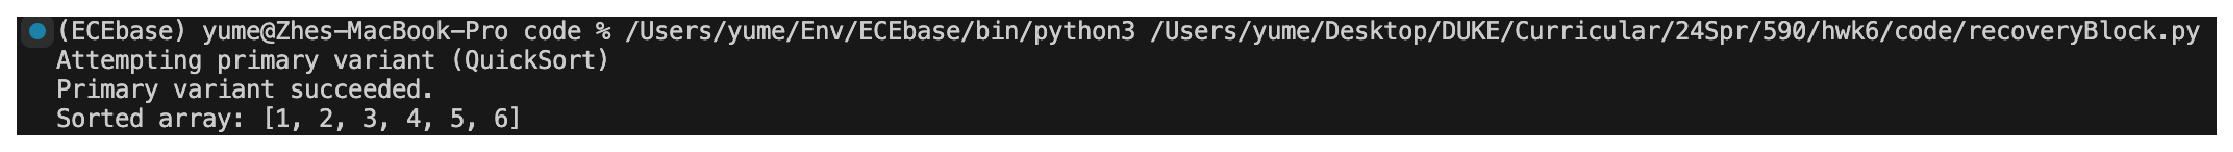
\includegraphics[width=1\textwidth]{image/1.eps}
\end{center}

This indicates that QuickSort was able to sort the array without any issues, and there was no need to attempt sorting with the alternate variant.

\textbf{If QuickSort Fails and InsertionSort Succeeds}: We can change line 5 to be: 

	\begin{lstlisting}[language=python]
left = [x for x in arr if x > pivot]\end{lstlisting} 

If the primary variant (QuickSort) fails to sort the array correctly, the program proceeds with the alternate variant (InsertionSort). If InsertionSort then successfully sorts the array, the output is:

\begin{center}
	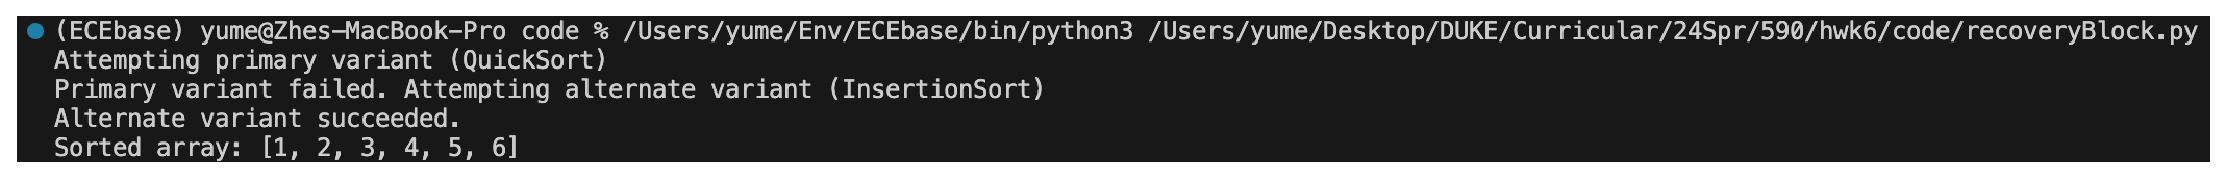
\includegraphics[width=1\textwidth]{image/2.eps}
\end{center}

This output demonstrates the recovery block scheme's ability to revert to an alternate sorting method upon the failure of the primary method, ensuring the task's completion.

\textbf{If Both QuickSort and InsertionSort Fail}: We can change line 14 to be: 

	\begin{lstlisting}[language=python]
while j ==0 and key < arr[j] :\end{lstlisting} 

 In the unlikely event that both QuickSort and InsertionSort fail to sort the array correctly, the program will raise an exception to indicate the failure of the recovery process, with the output being:

\begin{center}
	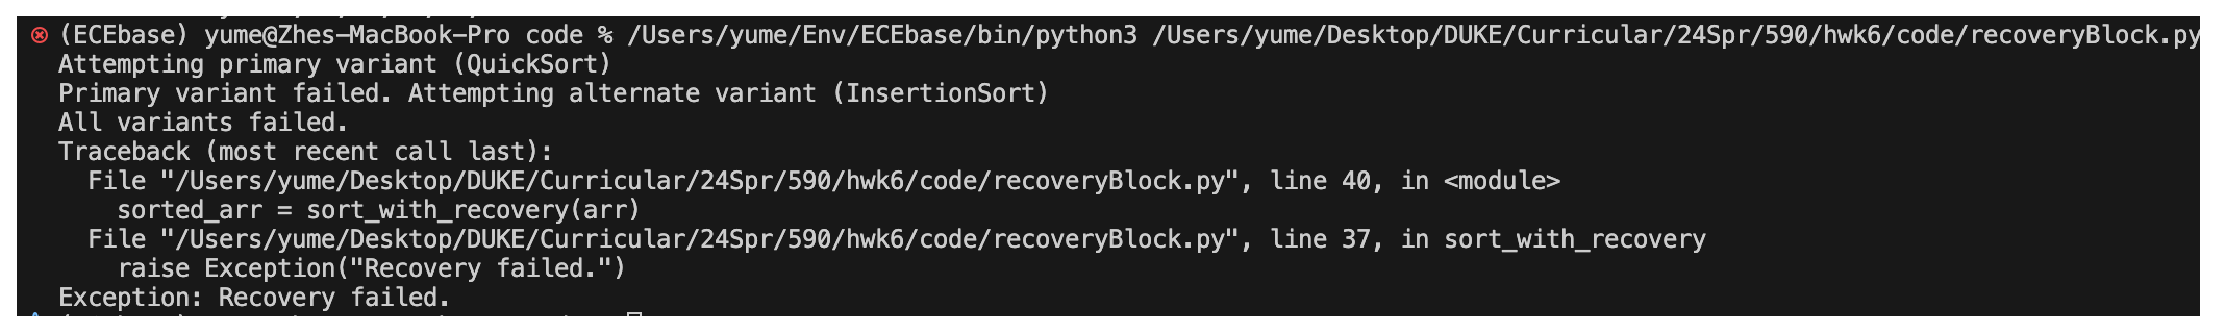
\includegraphics[width=1\textwidth]{image/3.eps}
\end{center}

This indicates a complete failure of the sorting process, where neither the primary nor the alternate sorting methods were able to produce a correctly sorted array, leading to the raising of an exception.




\end{document}
